\chapter{Проектирование приложения} \label{chapt2}

\section{Общий вид приложения} \label{sect2_1}

Чтобы представить общий вид приложения следует вернуться к поставленным задачам:

\begin{itemize}
  \item Переключение между различными ролями в RTK системе;
  \item Возможность изменять настройки основных режимов работы;
  \item Работа с конфигурационными файлами(создание, копирование, удаление);
  \item Отображение статуса системы - текущие координаты, качество решения;
  \item График уровней приема сигнала спутников;
  \item Список логов ГНСС данных с возможностью их скачать;
  \item Конвертация логов ГНСС данных в формат RINEX;
\end{itemize}

Следует разбить эти задачи на группы. К примеру, цель одних - отображение результата работы RTKLIB, цель других - изменение настроек. Также есть вспомогательные, но необходимые для нормальный работы задачи, такие как хранение, организация и скачивание логов. К задачам отображения следует отнести статус системы и график уровней приема спутников, очень полезный при установке антенны. К настройкам - переключение между ролями базы и ровера и, собственно, настройки этих самых ролей.

\clearpage

Как было видно из предыдущей главы, разбиение веб-страницы на тематические разделы - ход, на который пошла как большая компания, так и проект с открытым исходным кодом, поддерживаемый сообществом. Здесь это также представляется удобным ходом. Для разграничения различных областей приложения можно использовать стандартные для мобильных приложений вкладки(рис. 2.1).

\begin{figure}[ht]
  \center
  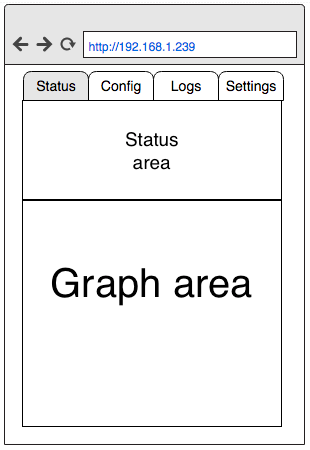
\includegraphics [scale=0.5] {General_mockup}
  \caption{Навигация внутри приложения}
  \label{img:latex}
\end{figure}

\clearpage

\section{Вкладки приложения} \label{sect2_2}

\subsection{Status} \label{subsect2_2_1}

В статус следует поставить информацию о координате, RTK режиме, статусе RTK решения. Кроме этого на один экран можно уместить и график с уровнями приема спутников. На рисунке 2.2 изображен набросок вкладки со статусом.

\begin{figure}[ht]
  \center
  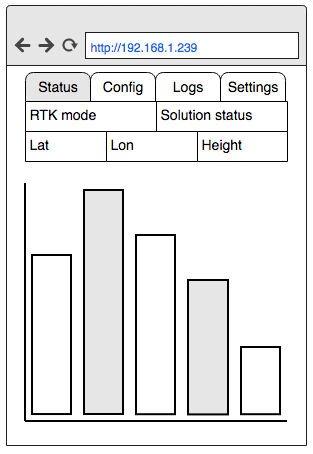
\includegraphics [scale=0.5] {Status_mockup}
  \caption{Статус приемника}
  \label{img:latex}
\end{figure}

\clearpage

\subsection{Config} \label{subsect2_2_2}

Вкладка конфигурации должна содержать возможность переключаться с базы на ровер и обратно. Кроме этого, нужно отображать настройки соответствующего режима. В случае с ровером должен быть выбор, какой конфигурационный файл использовать. На рисунке 2.3 изображен примерный вид вкладки конфигурации.

\begin{figure}[ht]
  \center
  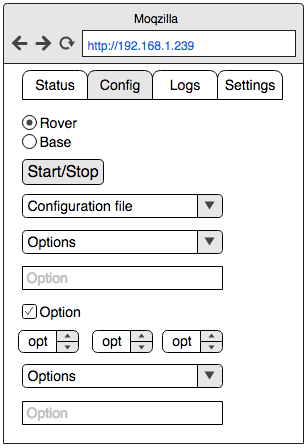
\includegraphics [scale=0.5] {Config_mockup}
  \caption{Конфигурация}
  \label{img:latex}
\end{figure}

\clearpage

\subsection{Logs} \label{subsect2_2_3}

Вкладка с логами будет содержать список логов(рис. 2.4). Удобнее всего логи сортировать по дате, но в обратном порядке. По нажатию на элемент такого списка, будет начинаться загрузка. Каждый элемент списка может содержать информацию о времени начала лога, формате и размере.

\begin{figure}[ht]
  \center
  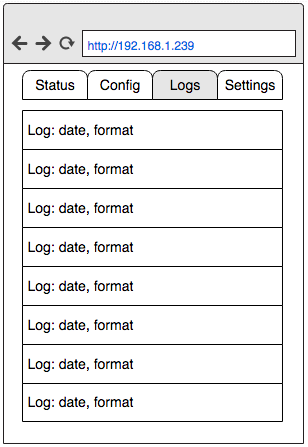
\includegraphics [scale=0.5] {Logs_mockup}
  \caption{Логи на устройстве}
  \label{img:latex}
\end{figure}

\clearpage

\subsection{Settings} \label{subsect2_2_4}

Здесь будут находиться настройки самого приложения: указание текущей версии и возможность обновления, выбор версии формата RINEX для конвертации логов, кнопка перезагрузки устройства. Набросок вкладки настроек - на рисунке 2.5

\begin{figure}[ht]
  \center
  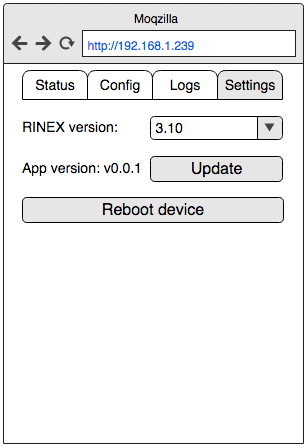
\includegraphics [scale=0.5] {Settings_mockup}
  \caption{Настройки приложения}
  \label{img:latex}
\end{figure}

\clearpage

\section{Взаимодействие с RTKLIB} \label{sect2_3}

Одним из сложных вопросов, которые следует решить при проектировании приложения - как наладить обмен информацией с программами RTKLIB. Существуют следующие варианты решения проблемы:

\begin{enumerate}
  \item Дописать приложение и серверную часть на языке C
  \item Дописать в RTKLIB передачу данных в механизм IPC уровня операционной системы и читать полезную информацию из стороннего приложения-сервера
  \item Запускать приложения RTKLIB в контролируемом контейнере, имитирующем запуск человеком в терминале
\end{enumerate}

Дело в том, приложения пакета написаны на C, а это не самый подходящий язык для написания веб-приложения. Существуют соответствующие фрэймворки и для языка C, но это скорее исключения из правил.

Еще одним важным аспектом, который нельзя не принять во внимание - общий стиль реализации проекта. Дело в том, что RTKLIB написан излишне сложно. Вот, например, выдержка из кода проекта:

\lstinputlisting[
  label={listings:rtklib_code_snippet},
  caption={Пример исходного кода RTKLIB},
  style={java}
]
{src/rtklib_code_snippet.c}

Наиболее простым и наиболее надежным способом работы с приложениями RTKLIB будет не вмешиваться в код проекта и не дописывать новую функциональность прямо в код приложений, а сделать обертку вокруг собранных исполняемых файлов. Под «оберткой» следует понимать запуск приложения в контролируемой среде, чтение и парсинг стандартного вывода, запись команд в стандартный ввод. Это позволит:

\begin{itemize}
  \item Не вмешиваться в сложную внутреннюю структуру приложения, рискуя что-то нарушить
  \item Сохранить совместимость с новыми версиями RTKLIB, даже при серьезных изменения кодовой базы
  \item Писать веб-приложение на более подходящем для этого языке
  \item Не добавлять никакие дополнительные механизмы IPC в RTKLIB
\end{itemize}

% \clearpage

\section{Общая архитектура и выбор инструментов разработки} \label{sect2_4}

Перед переходом к следующему этапу важно определиться с инструментами разработки - языком программирования и основными библиотеками. Так как основа всего проекта - веб-приложение, следует выбрать язык с популярным и функциональным фрэймворком для веб-разработки. Также, языку требуется наличие библиотеки для запуска внешних программ в контролируемом контейнере, как описано в предыдущей главе. Не следует забывать о том, что приложение будет запускаться на встраиваемом модуле с ограниченными параметрами производительности. Эти черты пересекаются в языке Python, дополненном библиотекой Pexpect и фрэймворком Flask, а также Ruby, дополненном фрэймворков Ruby on Rails и библиотекой RubyExpect. Оценим достоинства и недостатки этих подходов.

Первое, на что следует обратить внимание - проработанность ключевой библиотеки автоматизации исполняемых файлов - Pexpect и RubyExpect соответственно. Проект Pexpect \cite{pexpect-docs} существует уже более пяти лет, успешно и быстро развивается. На момент написания данной работы, доступна версия 4.1. RubyExpect же - гораздо более молодой проект с меньшей базой пользователей и функциональностью \cite{rubyexpect-docs}, что говорит в пользу языка Python.

Во-вторых, чтобы добиться ощущения мобильного приложения, можно сделать приложение одностраничным(реализовав вкладки внутри одной из страниц), а любые взаимодействия с сервером, кроме загрузки самой страницы, проводить через технологию WebSockets. Популярной Javascript библиотекой для работы с WebSockets является Socket.IO. Со стороны сервера Socket.IO полностью поддерживается расширением Flask под названием Flask-Socketio \cite{flask-socketio-docs}, разработанным Мигелем Гринбергом. Гринберг - опытный специалист в веб-разработке, написавший книгу по Flask, и его проект крайне популярен. В то же время, в Ruby on Rails полноценной поддержки Socket.IO нет.

Еще одним фактором при выборе языка разработки является наличие интерпретатора Python в сборке Linux на Emlid Reach, что сократит подготовительную работу.

Учитывая лучшую поддержку необходимых технологий, для разработки серверной части был выбран язык Python.

При создании веб-страницы, помимо библиотеки для работы с веб-сокетами, можно ограничиться стандартными инструментами - HTML, библиотеки jQuery \cite{jQuery} для манипуляций над элементами DOM. Также, для адаптивности страницы нужен подходящий набор элементов пользовательского интерфейса для создания самой страницы. Такой UI фрэймворк обеспечит работу приложения для практически любого браузера, на экранах самых разных размеров. Был выбран jQuery Mobile \cite{jQuery-mobile} позволяющий модифицировать стандартные элементы HTML страницы добавлением правильных свойств.

\clearpage

Результат работы, общий план архитектуры приложения можно увидеть на рисунке 2.6. Таким образом, для достижения поставленных целей предстоит разработать:

\begin{itemize}
  \item Модуль-сервер, обрабатывающий HTTP и WebSocket события;
  \item Модуль автоматизации работы с RTKLIB;
  \item HTML страницу, служащую интерфейсом пользователя;
  \item Модуль-клиент WebSocket события в браузере;
  \item Модуль работы с графиком;
\end{itemize}

\begin{figure}[ht]
  \center
  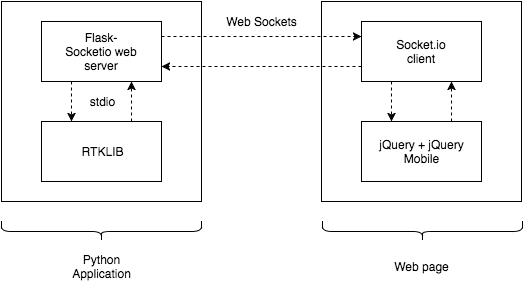
\includegraphics [scale=0.6] {App_architecture}
  \caption{Общий план архитектура приложения}
  \label{img:latex}
\end{figure}














